\section{Automated Building of Lab Environment on Kali Linux}
\label{apx:lab-final_envbuild}

For the second assignment for my Lab \textit{Host} system I choosed to use \textit{Kali Linux}\cite{os.kali}. 

The original documentation (please refer to: \cite{seedlab2024}) is referring to a pre-built \lstinline{*.iso} image denoted as \textit{Seed VM} which is based on the linux distribution Ubuntu (please refer to: \url{https://hub.docker.com/_/ubuntu}).  Since I'm not familiar with how they compiled the kernel nor which kernel modules are included or not in their custom Ubuntu container I built my own lab environment with slightly customization of the provided yml file \textit{docker-compose.yml} using Alpine Linux as a base for my container images.  For the container building process I used the tool called \textit{podman}\cite{podman}.

Podman is a daemonless, open source, Linux native tool designed to make it easy to find, run, build, share and deploy applications using Open Containers Initiative (OCI)\cite{oci.containers} Containers and Container Images.\cite{podman} Similarly to other common Container Engines (Docker, CRI-O, containerd), Podman relies on an OCI compliant Container Runtime (runc, crun, runv, etc) to interface with the operating system and create the running containers.\cite{podman} For the basic tasks we are able to simply make an alias to Docker to Podman (alias docker=podman) without any problems. 

\subsection{Cleanup the existing environment}

The \lstinline{VPN_LAB.yml} will build the whole lab environment from scratch, meaning that first the existing container images and networks should be removed:

\begin{lstlisting}[language=bash, caption=Host preparation for building the environment]
echo 'Delete previously created networks'
docker network rm --force "net-10.9.0.0"
docker network rm --force "net-192.168.50.0"
docker network rm --force "net-192.168.60.0"

echo 'Delete previously created containers'
docker stop host-192.168.50.5
docker stop host-192.168.50.6
docker stop host-192.168.60.5
docker stop host-192.168.60.6
docker stop host-vpn-server-10.9.0.11
docker stop host-client-server-10.9.0.12

docker rm host-192.168.50.5
docker rm host-192.168.50.6
docker rm host-192.168.60.5
docker rm host-192.168.60.6
docker rm host-vpn-server-10.9.0.11
docker rm host-client-server-10.9.0.12
\end{lstlisting}

Even tough in some cases if the container building process fails, some commit remains, this should be removed as well with \lstinline{docker image rm} command as can be seen of \textit{Figure \ref{fig:rmcon}}:

\begin{figure}[h]
    \centering
    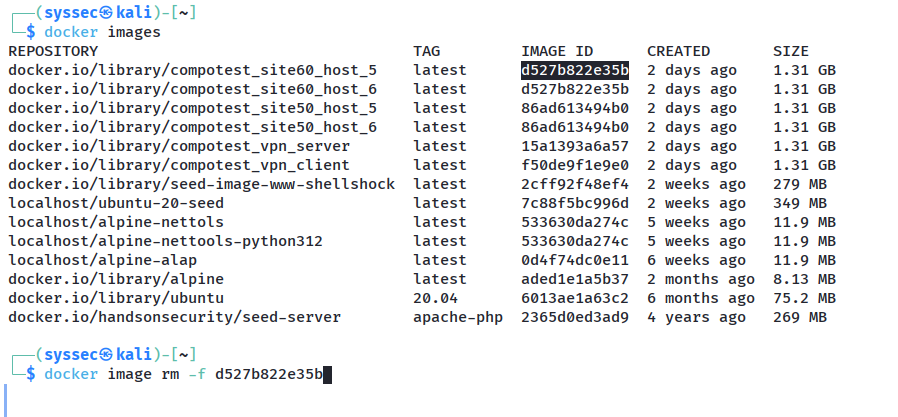
\includegraphics[width=0.5\linewidth]{Picture/00_Lab-Environment_Setup/999_docker-image-rm.png}
    \caption{Removing unnecessary container images}
    \label{fig:rmcon}
\end{figure}



\subsection{Review of \textit{Dockerfiles}\cite{docker.dockerfiles}}
\label{apx:lab-final_dockerfiles}

A \lstinline{Dockerfile} is basically a text document that contains all the necessary commands to call on the command line to assemble an image. For this specific lab I assembled four files according the network topology: \lstinline{Clientfile}, \lstinline{Serverfile}, \lstinline{SiteA}, \lstinline{SiteB} As an example I'll show snippets related to the container \lstinline{vpn-server-10.9.0.12}, but for a more comprehensive overview, please see the actual files I provided for the Assignment.

\subsubsection{Serverfile}
\label{apx:dockerfile.serverfile}

\begin{lstlisting}[language=bash,caption=Serverile overview for container vpn-server-10.9.0.11]
# ===========================================================
# Dockerfile for Building: VPN_SERVER
# ===========================================================

# Define container image
FROM alpine:latest

# Refresh repository
RUN apk update

# Install base packages
RUN apk add --no-cache busybox-extras tcpdump  texlive \
        tshark  graphviz  imagemagick  libpcap libpcap-dev \
        xdg-utils  openssl  openssl-dev   \
        graphviz imagemagick  sox  gcc  autoconf \
        curl vim nano python3 scapy iptables ca-certificates

# Install python3 and pip related packages
RUN apk add --no-cache python3 py3-matplotlib py3-cryptography python3-dev py3-pip

# Create python virtual environment
RUN python3 -m venv /opt/venv
COPY requirements.txt requirements.txt
RUN . /opt/venv/bin/activate && pip install -r requirements.txt

# Set server's listening port according to `tls_server.py`
EXPOSE 8443

WORKDIR /home/
COPY 00_keygen.sh /home/00_keygen.sh
COPY cert.conf /home/cert.conf
RUN chmod +x /home/00_keygen.sh
COPY tls_server.py /home/tls_server.py
RUN chmod +x /home/tls_server.py

# Add routing according to network topology
CMD ["/bin/ash", "ip route del default"]
CMD ["/bin/ash", "ip route add default via 10.9.0.1"]
CMD ["/bin/ash", "ip route add 192.168.60.0 via 192.168.60.11"]

# Build tunnel and tls client/server
#ENTRYPOINT ["python", "/home/tls_server.py", "--debug"]

\end{lstlisting}


\subsubsection{Clientfile}
\label{apx:dockerfile.clientfile}

The following code-snippet shows the \textit{Dockerfile} for automating the build process of \lstinline{vpn-client-10.9.0.12}

\begin{lstlisting}[language=bash, caption=Clientfile overview for container vpn-client-10.9.0.12]
# ===========================================================
# Dockerfile for Building: VPN_CLIENT
# ===========================================================

# Define container image
FROM alpine:latest

# Refresh repository
RUN apk update

# Install base packages
RUN apk add --no-cache busybox-extras tcpdump  texlive \
        tshark  graphviz  imagemagick  libpcap libpcap-dev \
        xdg-utils  openssl  openssl-dev   \
        graphviz imagemagick  sox  gcc  autoconf \
        curl vim nano python3 scapy iptables ca-certificates

# Install python3 and pip related packages
RUN apk add --no-cache python3 py3-matplotlib py3-cryptography python3-dev py3-pip

# Create python virtual environment
RUN python3 -m venv /opt/venv
COPY requirements.txt requirements.txt
RUN . /opt/venv/bin/activate && pip install -r requirements.txt

# Set server's listening port according to `tls_server.py`
EXPOSE 8443

WORKDIR /home/
COPY 00_keygen.sh /home/00_keygen.sh
COPY cert.conf /home/cert.conf
RUN chmod +x /home/00_keygen.sh
COPY tls_client.py /home/tls_client.py
RUN chmod +x /home/tls_client.py

# Add routing according to network topology
CMD ["/bin/ash", "ip route del default"]
CMD ["/bin/ash", "ip route add default via 10.9.0.1"]
CMD ["/bin/ash", "ip route add 192.168.50.0 via 192.168.50.12"]

# Build tunnel and tls client/server
#ENTRYPOINT ["python", "/home/tls_client.py", "--debug"]

\end{lstlisting}

\subsubsection{SiteA}

\begin{lstlisting}[language=bash, caption=Overview of SiteA dockerfile for containers within the subnet 192.168.50.0/24]
# ===========================================================
# Dockerfile for Building: SITE_A (192.168.50.0/24)
# ===========================================================

# Define container image
FROM alpine:latest

# Refresh repository
RUN apk update

# Install base packages
RUN apk add --no-cache busybox-extras tcpdump  texlive \
        tshark  graphviz  imagemagick  libpcap libpcap-dev \
        xdg-utils  openssl  openssl-dev   \
        graphviz imagemagick  sox  gcc  autoconf \
        curl vim nano python3 scapy iptables ca-certificates

# Install python3 and pip related packages
RUN apk add --no-cache python3 py3-matplotlib py3-cryptography python3-dev py3-pip

# Create python virtual environment
RUN python3 -m venv /opt/venv
COPY requirements.txt requirements.txt
RUN . /opt/venv/bin/activate && pip install -r requirements.txt

# Add routing according to network topology
CMD ["/bin/ash", "ip route del default"]
CMD ["/bin/ash", "ip route add default via 192.168.50.12"]
CMD ["/bin/ash", "ip route add 192.168.60.0/24 via 192.168.50.12"]

# Generate keys/certificates
WORKDIR /home/
COPY 00_keygen.sh /home/00_keygen.sh
COPY cert.conf /home/cert.conf
RUN chmod +x /home/00_keygen.sh

\end{lstlisting}

\subsubsection{SiteB}
\begin{lstlisting}[language=bash, caption=Overview of SiteB dockerfile for containers within subnet 192.168.60.0/24]
# ===========================================================
# Dockerfile for Building: SITE_B (192.168.60.0/24)
# ===========================================================

# Define container image
FROM alpine:latest

# Refresh repository
RUN apk update

# Install base packages
RUN apk add --no-cache busybox-extras tcpdump  texlive \
        tshark  graphviz  imagemagick  libpcap libpcap-dev \
        xdg-utils  openssl  openssl-dev   \
        graphviz imagemagick  sox  gcc  autoconf \
        curl vim nano python3 scapy iptables ca-certificates

# Install python3 and pip related packages
RUN apk add --no-cache python3 py3-matplotlib py3-cryptography python3-dev py3-pip

# Create python virtual environment
RUN python3 -m venv /opt/venv
COPY requirements.txt requirements.txt
RUN . /opt/venv/bin/activate && pip install -r requirements.txt

# Add routing according to network topology
CMD ["/bin/ash", "ip route del default"]
CMD ["/bin/ash", "ip route add default via 192.168.60.11"]
CMD ["/bin/ash", "ip route add 192.168.50.0/24 via 192.168.60.11"]

# Generate keys/certificates
WORKDIR /home/
COPY 00_keygen.sh /home/00_keygen.sh
COPY ca.conf /home/ca.conf
RUN chmod +x /home/00_keygen.sh

\end{lstlisting}

\subsubsection{Overview of requirements.txt}

\begin{lstlisting}[language=python, caption=Overview of requirements.txt]
    alabaster==1.0.0
astroid==3.3.9
asttokens==3.0.0
babel==2.17.0
certifi==2025.1.31
cffi==1.17.1
charset-normalizer==3.4.1
contourpy==1.3.1
cryptography==44.0.2
cycler==0.12.1
decorator==5.2.1
dill==0.3.9
docutils==0.21.2
executing==2.2.0
fonttools==4.56.0
graphviz==0.20.3
idna==3.10
imagesize==1.4.1
ipython==9.0.2
ipython_pygments_lexers==1.1.1
isort==6.0.1
jedi==0.19.2
Jinja2==3.1.6
kiwisolver==1.4.8
MarkupSafe==3.0.2
matplotlib==3.10.1
matplotlib-inline==0.1.7
mccabe==0.7.0
numpy==2.2.3
p0f==1.0.0
packaging==24.2
parso==0.8.4
pexpect==4.9.0
pillow==11.1.0
platformdirs==4.3.7
prompt_toolkit==3.0.50
ptyprocess==0.7.0
pure_eval==0.2.3
pycparser==2.22
pycryptodome==3.22.0
Pygments==2.19.1
pylint==3.3.6
pyparsing==3.2.1
python-dateutil==2.9.0.post0
PyX==0.16
pyxi==0.1.4
requests==2.32.3
roman-numerals-py==3.1.0
setuptools==78.1.0
six==1.17.0
snowballstemmer==2.2.0
Sphinx==8.2.3
sphinx-rtd-theme==3.0.2
sphinxcontrib-applehelp==2.0.0
sphinxcontrib-devhelp==2.0.0
sphinxcontrib-htmlhelp==2.1.0
sphinxcontrib-jquery==4.1
sphinxcontrib-jsmath==1.0.1
sphinxcontrib-qthelp==2.0.0
sphinxcontrib-serializinghtml==2.0.0
stack-data==0.6.3
tinyec==0.4.0
tomlkit==0.13.2
traitlets==5.14.3
urllib3==2.3.0
wcwidth==0.2.13
wheel

\end{lstlisting}


\subsection{Review of \textit{VPN\_LAB.yml} file}
The container environment can be built automatically with the following \lstinline{.yml} file, with command: \lstinline{podman compose --file VPN_LAB.yml up --force-recreate --detach}


\begin{lstlisting}[language=bash, caption=Building lab environment based on VPN\_LAB.yml]
version: "3"

services:
    vpn_client:
        build:
            context: .
            dockerfile: Clientfile
        container_name: vpn-client-10.9.0.12
        tty: true
        cap_add:
                - ALL
        devices:
                - "/dev/net/tun:/dev/net/tun"
        sysctls:
                - net.ipv4.ip_forward=1
        volumes:
                - ./volumes:/volumes
        networks:
            net-10.9.0.0:
                ipv4_address: 10.9.0.12
            net-192.168.50.0:
                ipv4_address: 192.168.50.12
        command: ash -c "source ./00_keygen.sh && host_keygen client && host_keygen server && inetd start && tail -f /dev/null"

    vpn_server:
        build:
            context: .
            dockerfile: Serverfile
        container_name: vpn-server-10.9.0.11
        tty: true
        cap_add:
                - ALL
        devices:
                - "/dev/net/tun:/dev/net/tun"
        sysctls:
                - net.ipv4.ip_forward=1
        volumes:
                - ./volumes:/volumes
        networks:
            net-10.9.0.0:
                ipv4_address: 10.9.0.11
            net-192.168.60.0:
                ipv4_address: 192.168.60.11
        command: ash -c "source ./00_keygen.sh && host_keygen client && host_keygen server && inetd start && tail -f /dev/null"

    site50_host_5:
        build:
            context: .
            dockerfile: SiteA
        container_name: host-192.168.50.5
        tty: true
        cap_add:
                - ALL
        networks:
            net-192.168.50.0:
                ipv4_address: 192.168.50.5
        command: ash -c "source ./00_keygen.sh && host_keygen client && inetd start && tail -f /dev/null"

    site50_host_6:
        build:
            context: .
            dockerfile: SiteA
        container_name: host-192.168.50.6
        tty: true
        cap_add:
                - ALL
        networks:
            net-192.168.50.0:
                ipv4_address: 192.168.50.6
        command: ash -c "source ./00_keygen.sh  && host_keygen client && inetd start && tail -f /dev/null"

    site60_host_5:
        build:
            context: .
            dockerfile: SiteB
        container_name: host-192.168.60.5
        tty: true
        cap_add:
                - ALL
        networks:
            net-192.168.60.0:
                ipv4_address: 192.168.60.5
        command: ash -c "source ./00_keygen.sh  && host_keygen client && inetd start && tail -f /dev/null"

    site60_host_6:
        build:
            context: .
            dockerfile: SiteB
        container_name: host-192.168.60.6
        tty: true
        cap_add:
                - ALL
        networks:
            net-192.168.60.0:
                ipv4_address: 192.168.60.6
        command: ash -c "source ./00_keygen.sh  && host_keygen client && inetd start && tail -f /dev/null"

networks:
    net-192.168.50.0:
        name: net-192.168.50.0
        ipam:
            config:
                - subnet: 192.168.50.0/24
    net-192.168.60.0:
        name: net-192.168.60.0
        ipam:
            config:
                - subnet: 192.168.60.0/24

    net-10.9.0.0:
        name: net-10.9.0.0
        ipam:
            config:
                - subnet: 10.9.0.0/24


\end{lstlisting}